\documentclass{VUMIFPSbakalaurinis}
\usepackage{algorithmicx}
\usepackage{algorithm}
\usepackage{algpseudocode}
\usepackage{amsfonts}
\usepackage{amsmath}
\usepackage{bm}
\usepackage{caption}
\usepackage{color}
\usepackage{float}
\usepackage{graphicx}
\usepackage{listings}
\usepackage{subfig}
\usepackage{wrapfig}
\usepackage{listings}

\lstset {
  language=Scala,
  basicstyle=\footnotesize,
  numbers=left,
  stepnumber=1,
  showstringspaces=false,
  tabsize=1,
  breaklines=true,
  breakatwhitespace=false,
}

% Titulinio aprašas
\university{Vilniaus universitetas}
\faculty{Matematikos ir informatikos fakultetas}
\institute{Informatikos institutas}  % Užkomentavus šią eilutę - institutas neįtraukiamas į titulinį
\department{Programų sistemų bakalauro studijų programa}
\papertype{Bakalauro baigiamasis darbas}
\title{Translation Unit Granularization}
\titleineng{Kompiliatoriaus transliuojamo vieneto smulkinimas}
\author{Andrius Bentkus}
% \secondauthor{Vardonis Pavardonis}   % Pridėti antrą autorių
\supervisor{asist. dr. Vytautas Valaitis}
\reviewer{doc. dr. Vardauskas Pavardauskas}
\date{Vilnius – \the\year}

% Nustatymai
% \setmainfont{Palemonas}   % Pakeisti teksto šriftą į Palemonas (turi būti įdiegtas sistemoje)
\bibliography{bibliografija}

\begin{document}
\maketitle

%% Padėkų skyrius
% \sectionnonumnocontent{}
% \vspace{7cm}
% \begin{center}
%     Padėkos asmenims ir/ar organizacijoms
% \end{center}

\sectionnonumnocontent{Summary}
This thesis presents an approach on how to speed up compilation in a day to day programming scenario, benchmarks the performance improvements with various inputs and compares the gathered performance metrics to an already existing compiler.

Classic compilers treat a source file as an atomic translation unit in their compilation pipeline, the proposed approach tries to leverage the structure of modern programming languages to granularize the translation unit in order to improve recompilation times for classic development workloads.

The chosen target language is a subset of the Scala programming language.
Instead of modifying the standard Scala compiler to accommodate the proposed approach, a compiler is written from scratch in order to have simple program enabling straightforward modifications for an easier accommodation of the proposed approach.

Performance measurements of the prototype compiler are taken with the approach enabled and disabled, various dynamic inputs are generated with different compilation unit sizes to gain insights in the effectiveness of the approach.
Results are then compared to the classic compiler and conclusions are drawn.

\keywords{Compilers, Translation Unit, Compiler optimization}

\sectionnonumnocontent{Santrauka}
% TODO: translation in lithuanian

% Nurodomi iki 5 svarbiausių temos raktinių žodžių (terminų).
% Vienas terminas gali susidėti iš kelių žodžių.
\raktiniaizodziai{Transliavimas, Transliavimo optimizacijos}


\tableofcontents

\sectionnonum{Introduction}

%\subsectionnonum{Overview}
%\subsectionnonum{Contributions}
%\subsectionnonum{Outline}

\subsectionnonum{Research object and actuality}
The majority of the research done on compilers is focused on making compilers output optimized programs in terms of code execution speed and memory usage \cite{lopes2018future} while neglecting or willfully sacrificing \cite{fast2019compilers} actual runtime performance of the compiler itself.
As computers get faster more resources are available, but programmers tend to utilize these newfound resources to make the implementation of programs simpler rather than making the programs faster\cite{Wirth1995}.

Another vector of academic improvement within the compiler sphere is to add new features or utilize paradigms like dependent types or formal specifications\cite{RustVerification} in order to allow the compiler to do more sophisticated type checking and verification than classic type checking allows while significantly increasing runtime compilation .

% ecosystem is bad
When assessing the adoption of a new programming language the runtime speed of the available compilers for a particular programming languages are often gauged as an important metric\cite{ScalaSlow} among other such as language complexity, available libraries and spread of ecosystem.
Dealing with enormous compilation times of huge projects can have negative effects on the productivity of programmers and even drive away people from an entire ecosystem \cite{ScalaReallySlow, ScalaSlow}.

Modern organizations moving towards continuous delivery practices called DevOps \cite{DevOps} experience an ever increasing need to run the compilations over and over within their CI pipeline.
% todo: change mantra maybe
Slow compilation speeds go against the very mantra of the short cycle times promoted in DevOps and has spurred creation and adoption of minimal programming language focused on compilation speed and productivity to counter the effects of giant code bases on the CI process\cite{TheGoProgrammingLanguage, GoGoogle}.

\subsectionnonum{Goal}
This thesis will analyze the effects of compilation unit granularization in a compiler on the compilation speed.

It will be achieved by the following tasks:

\begin{enumerate}
\item{Creation of a compiler.}
\item{Implementation of compilation unit granularization.}
\item{Correctness validation for the compiler.}
\item{Measurements of the impact on performance.}
\item{A performance comparison to existing compilers.}
\end{enumerate}

The expected results will be a compiler with compilation unit granularization and various performance measurements together with a comparison to an existing compiler.

\subsectionnonum{Challenges and expected results}
The goal of this bachelor thesis is to create a prototype compiler for a small subset of the Scala programming language.
Since writing a compiler is a difficult task in itself and Scala is known to have a multitude of advanced and complicated features\cite{ScalaSpec}, the targeted compiler implementation in this thesis will support only basic features in order to allow for an easier realization of the proposed augmentation to the compiler.

% todo: introduced errors?
When writing software developers tend to create only small changes in existing source files before running the compilation again for a quick feedback loop of introduced errors.
A translation unit is the entire input of source code that is used to produce a compilation output and is usually reprocessed in its entirety without consideration of previous outputs compilation outputs, hence even small changes in a giant class requires a complete recompilation of the entire class which might be costly if the codebase is large.

The core idea of the thesis is to granularize the translation unit size order to increase performance of subsequent compilations of the same source file with minimal source modifications to allow for an measurable speed improvement in this kind of feedback loop.

Such granularization requires additional compiler logic and might overcomplicate an already sophisticated computer program.
Additional challenges might arise when ensuring compilation output correctness and preserving compilation output similarity.
The lack of complex compiler features in the prototype might skew the results against the advantages of granularization since complex compiler features incur the most significant compilation runtime penalties.

% Tyrimo Metodas
\subsectionnonum{Investigation method}
Time measurements in the millisecond range will be taken of subsequent compilation runs changing only parts of the source code using the prototype compiler written in this thesis with the translation unit granularization feature enabled and disabled.

Various source code input sizes and complexity of source code will be evaluated.
A classic looking case study of average code complexity will be chosen, emphasized, discussed and evaluated, for example, a translation unit with 5 classes and 10 methods in every class with a small change in a singular method between compilations and another measurement with a small change in a singular class.

An automated but definitive and consistent source code generation tool will be used to create consistently reproducible results for the given inputs listed in the following list.

\section{Translation Unit}
The classic approach of compilers is to read an entire source file and generate a corresponding output file with the translated code.

For example in C++ and C source files with the extensions .cpp or .c are compiled to an intermediate object file with the extension .o, containing the generated assembly code of a specific target architecture, x86, ARM, etc.
Once all source files are compiled into object files, all object files are combined together with optional resources into a singular output file called the executable.

The Java language forces the programmer to define every Java class in its own file and every .java file is then compiled to a .class file, which can be later packaged to .jar files together with additional resources for easier deployment.
A .class file contains all the Java bytecode generated from the Java source file, a condensed representation of the a Java class in a high level format which is abstract and does not target any specific target architecture, but an abstract architecture called the Java Virtual Machine (JVM).
Code targeting the JVM can be then executed provided a Java runtime is present on the target machine which Just in Time (JIT) compiles the bytecode to the target machines assembly code and executes it.

% todo: maybe later?
Java bytecode is much more abstract and conceptually closer to the original representation of a class than the generated object files containing assembly are.
Java class methods are basically sections in a .class file \cite{JvmMethods} which wrap Java bytecode - the implementation of the methods functionality.
This high level representation makes granularization of translation units much more convenient, because it is possible to map a method directly to an entire section within the class file.

Scala also targets the JVM, however it does not share the limitation of one class per source file that Java has.
A Scala source file can contain multiple class definitions in a singular and due to the possibility to define class in a very concise manner developers gravitate towards multiple class definitions per file \ref{multidef}.

% listings https://tex.stackexchange.com/questions/321843/using-labels-for-lstinputlisting

\lstinputlisting[language=Scala, linewidth=18cm, label={multidef}, caption={An interface and 3 class definitions in a singular source file}]{./code/Expression.scala}

The compiler creates in total 4 corresponding .class files as depicted in Listing \ref{img:Expression}.
The classes all depend on the same trait definition called Expression, which is an empty interface in Java called a Marker Interface \cite{10.5555/1407381}, however there is no need for a strict compilation order, the compiler can utilize the meta information to compile all result .class files in parallel or whatever order it sees fit.

When running the compiler with the source file displayed in \ref{multidef} as the input, the compiler will recompile all 4 classes, even though new modifications might be present only within one class because the minimal translation unit is the entire source file.
In the given examples the classes are trivial and the performance when recompiling is negligible.

\begin{figure}[H]
    \centering
    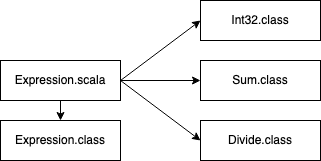
\includegraphics[scale=0.6]{img/Expression}
    \caption{Compilation result of Listing \ref{multidef}}
    \label{img:Expression}
\end{figure}

One might argue that multiple sizable class implementations with numerous methods contained in a singular source file are rare in actual code bases and optimizing for this case would yield minuscule benefits outside of tailored benchmarks, but the opposite is the truth. % todo: replace but a the opposite is true.
In the following example a typical usage of a popular Scala unit testing library Specs2 \cite{Specs2Github} is shown.

\lstinputlisting[language=Scala, linewidth=18cm, label={code:specs2code}, caption={Standard usage of Specs2}]{./specs2/SampleTest.scala}

Scala developers tend to use use many language features to create a Domain Specific Language (DSL) for visually pleasing code.
% TODO: maybe explain, but reword for sure
Because many Scala compiler feature are in play in this example, the details are quite intricate, but the result is that for each test case shown in the example \ref{code:specs2code} (first test, second test) a stand alone .class compilation output is created (SampleTest\$\$annon\$1.class, \$SampleTest\$\$anon\$2.class).
Having many unit tests in a sophisticated codebase can therefore prolong the compilation process significantly, to a point where an iterative development process becomes impractical.
Compilation times longer than a minute can be easily surpassed when meticulously writing Unit tests in a Test Drive Development (TDD) environment.

TDD also promotes writing tests as a playground to explore approaches and test code feasibility before writing the actual code, therefore long compilation times of unit tests can make such an approach impractical.
There are many reasons why such an optimization might improve usage of a compiler and increase the development experience of a developer.

\section{Compiler}
At the start of the bachelor thesis a thorough investigation was made to analyze how the official Scala compiler works \cite{ScalaGithub} and if it is feasible to apply the targeted optimizations to it.
The investigation took very long and yielded little results, the codebase was too humongous and complicated too understand, the compiler too featured packed to adjust with the target objectives.
Without the help of a mentor with high proficiency in the official Scala compiler codebase and taking the scope of the bachelor thesis into account, it was deemed too complicated to undergo such a task.

Instead of adjusting an already existing compiler, a compiler was written from scratch with an iterative approach.
In the following numerous advantages and disadvantages of this method are expressed.

\textbf{Flexibility} - big mature compilers are right and harder to change, they have accumulated a lot of code which needs to be adjusted for every modification.
The official Scala compiler has a complex pipeline with multiple passes and figuring out where what the best point of incision is a difficult task.
A small compiler written from scratch allows the author to focus on the most important aspects.

\textbf{Correctness} - ensuring that a new feature is correctly implemented in a sizable code base is an immense undertaking.
In order to ensure that a new feature addition doesn't impact the overall behavior of the compiler every feature needs to be tested for correctness.
The multi-pass nature of the official Scala compiler makes reasoning about correctness difficult, because it is a non trivial undertaking to reason about how caching in one pass might affect functionality the subsequent passes.

\textbf{Simplicitly and transparency} - a small compiler is simple and easy to reason about.
Writing one from scratch means that the entirity of the compiler is understood which enables better reasoning.
New features are easier to add because of a complete understanding.
Debugging is much more pleasant since the number of affected features is smaller.

\textbf{Accuracy} - the results might be skewed since it the self written compiler implements only a handful of features of the official language standard.
This can go both ways.

% todo: add references (
Some elaborate Scala features like type-driven implicits and mixing multiple traits are computationally very intensive.
The former needs to recurs in a nonterministic way on distinct implicit types in order to find a correct type inheritance path while the latter creates a proxy method in a target classes for every method within a mixed in non trivial trait.
Being able to reuse computation instead of redoing these kind of workloads might add significant performance boosts.

On the other hand, adding a multitude of features might slow down general compilation speeds of the compiler.
In ideal programming scenarios features that are not used but are implemented should not add any significant slow down to execution speeds, but code bases are rarely ideal.

\subsection{Implementation}
Creating a compiler from scratch for a non trivial small language is a significant task.
% todo: need citation?
Programming languages have become quite complex, containing multiple paradigms.
Each language feature on its on might look simple and be easy to understand but putting another cog in an already complex machine can prove to be difficult.

% todo: cite
Object Oriented Programming (OOP) has become quite obiquitess and is a base line feature that most of programming languages have.
Many developers are proefficient in at least one programming language supporting OOP and the most popular programming languages utilize OOP very prominently.

\subsection{Language}
The target compiler programming language is Scala.
%Scala mixes multiple OOP and functional programming paradigms extensively creating a feature rich environment for developers.
%Functions in Scala are values and all values are objects which
Scala mixes OOP and functional programming paradigm to create a feature rich environment for developers.
Functions in Scala are values and all values are objects, a smart way to seamlessly integrate both paradigms in a potent mix.

% https://data-flair.training/blogs/scala-features-comprehensive-guide/
The language aims to be concise and aesthetically pleasing utilizing features such as comprehensive type inference to minimize verbosity.
Functional aspects are prominently represented with a lightweight syntax for anonymous functions, higher order functions, currying, lazy evaluation, Algebraic Data Types (ADT), higher order functions, pattern matching.

% https://livebook.manning.com/book/scala-in-depth/chapter-10/3
% http://englishonlineclub.com/pdf/Scala%20in%20Depth%20[EnglishOnlineClub.com].pdf
Scala is a programming language targeting the Java Virtual Machine (JVM).
Running on the JVM allows Scala easily to utilzie existing Java code, which is a tremendous advantage because utilizing existing Java code opens access to a plathora of well maintained libraries targeting a wide range of needs.
The opposite however is not always true since Scala has a lot of features which can not be directly translated to JVM bytecode which is the underlying instruction set powering the JVM.

\sectionnonum{Results and conclusion}
\subsectionnonum{Results}
This is the result.



% (cituotų, perfrazuotų ar bent paminėtų) mokslo leidinių, kitokių publikacijų
% bibliografiniai aprašai. Šaltinių sąrašas spausdinamas iš naujo puslapio.
% Aprašai pateikiami netransliteruoti. Šaltinių sąraše negali būti tokių
% šaltinių, kurie nebuvo paminėti tekste. Šaltinių sąraše rekomenduojame
% necituoti savo kursinio darbo, nes tai nėra oficialus literatūros šaltinis.
% Jei tokių nuorodų reikia, pateikti jas tekste.

% \sectionnonum{Sąvokų apibrėžimai}
\sectionnonum{Acronyms}

\textbf{AST} - Abstract Syntax Tree

\textbf{JVM} - Java Virtual Machine

\textbf{JIT} - Just In Time

\textbf{DSL} - Domain Specific Language

\textbf{TDD} - Test Driven Development

\textbf{OOP} - Object Oriented Programming

\textbf{ADT} - Algebraic Data Type

\appendix  % Priedai
% Prieduose gali būti pateikiama pagalbinė, ypač darbo autoriaus savarankiškai
% parengta, medžiaga. Savarankiški priedai gali būti pateikiami ir
% kompaktiniame diske. Priedai taip pat numeruojami ir vadinami. Darbo tekstas
% su priedais susiejamas nuorodomis.

\section{Neuroninio tinklo struktūra}
\begin{figure}[H]
    \centering
    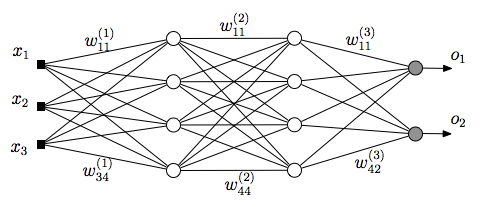
\includegraphics[scale=0.5]{img/MLP}
    \caption{Paveikslėlio pavyzdys}
    \label{img:mlp}
\end{figure}


\section{Eksperimentinio palyginimo rezultatai}
% tablesgenerator.com - converts calculators (e.g. excel) tables to LaTeX
\begin{table}[H]\footnotesize
  \centering
  \caption{Lentelės pavyzdys}
  {\begin{tabular}{|l|c|c|} \hline
    Algoritmas & $\bar{x}$ & $\sigma^{2}$ \\
    \hline
    Algoritmas A  & 1.6335    & 0.5584       \\
    Algoritmas B  & 1.7395    & 0.5647       \\
    \hline
  \end{tabular}}
  \label{tab:table example}
\end{table}

\printbibliography[heading=bibintoc]

\end{document}
